\documentclass{article}
\usepackage[utf8]{inputenc}
\usepackage[english]{babel}
\usepackage[margin=1in]{geometry}

\usepackage{fancyhdr}
\usepackage{extramarks}
\usepackage{amsmath}
\usepackage{amsthm}
\usepackage{amsfonts}
\usepackage{tikz}
\usepackage[plain]{algorithm}
\usepackage{algpseudocode}
\usepackage{arydshln}
\usepackage{mathtools}
\usepackage{cases}
\usepackage{listings}
\usepackage[numbered]{mcode}
\usepackage{booktabs}
\usepackage{graphicx}
\usepackage{subfigure}

\usepackage{blindtext}
\usepackage{amssymb}
\usepackage{hyperref}
\hypersetup{
    colorlinks=true,
    linkcolor=blue,
    filecolor=magenta,
    urlcolor=cyan,
}

\urlstyle{same}

%\newtheorem{theorem}{Theorem}
\newtheorem{theorem}{Theorem}[section]
\newtheorem{corollary}{Corollary}[theorem]
\newtheorem{lemma}[theorem]{Lemma}
\theoremstyle{remark}
\newtheorem*{remark}{Remark}

\theoremstyle{definition}
\newtheorem{definition}{Definition}[section]

\title{CS 250 - Computer Architecture \\ Homework 3 Written}
\author{Jincheng He Email: jincheng.he@dukekunshan.edu.cn}
\date{October 11, 2021}

\begin{document}

    \maketitle


    \section{Q1 Boolean Algebra}
    \begin{enumerate}
        \item[(a)] Write a truth table for the followgin function: $\text{Output} = \left( \left( !A + !B \right)\cdot !C \right) + \left( \left( A\cdot !B \right) + \left( !C\cdot B \right) \right)$.

        The result is as table~\ref{tab:Q1a_tt}.
        \begin{table}[!htbp]
            \centering
            \begin{tabular}{cccc}
                \toprule
                A & B & C & Output \\
                \midrule
                0 & 0 & 0 & 1      \\
                0 & 0 & 1 & 0      \\
                0 & 1 & 0 & 1      \\
                1 & 0 & 0 & 1      \\
                1 & 1 & 0 & 1      \\
                1 & 0 & 1 & 1      \\
                0 & 1 & 1 & 0      \\
                1 & 1 & 1 & 0      \\
                \bottomrule
            \end{tabular}
            \caption{Q1 (a) truth table.}
            \label{tab:Q1a_tt}
        \end{table}

        \item[(c)] Write a sum-of-products Boolean function for both outputs in the following truth table and then minimize them using Boolean logic, de Morgan's laws, etc.
        $$
        \begin{aligned}
            \text{out1} &= \left( A \& !B \& !C \right) | \left( A \& !B \& C \right) | \left( A \& B \& !C \right) \\
            &= \left( A \& !B \right) | \left( A \& B \& !C \right) \\
            &= A \& \left( !B | \left( B \& !C \right) \right) \\
            &= A \& \left( !B \& !C \right) \\
            &= A \& !\left( B | C \right)
        \end{aligned}
        $$

        $$
        \begin{aligned}
            \text{out2} &= \left( !A \& !B \& !C \right) | \left( !A \& B \& C \right) | \left( A \& B \& C \right) \\
            &= \left( !A \& !B \& !C \right) | \left( B \& C \right) \\
            &= !\left( A|B|C \right) | \left( B \& C \right)
        \end{aligned}
        $$

    \end{enumerate}


    \section{Q3 Finite State Machine}
    \begin{enumerate}
        \item[(a)] Draw a state transition diagram, where each state has a unique identifier that is a string of bits as well as the associated value for output \textbf{starter\_motor} and \textbf{ignition\_coil}. Label all of the arcs between transitions with the inputs \textbf{start\_engine} and \textbf{engine\_running} that cause those transitions.

        The answer is as figure~\ref{fig:diag}.
        \begin{figure}[!htbp]
            \centering
            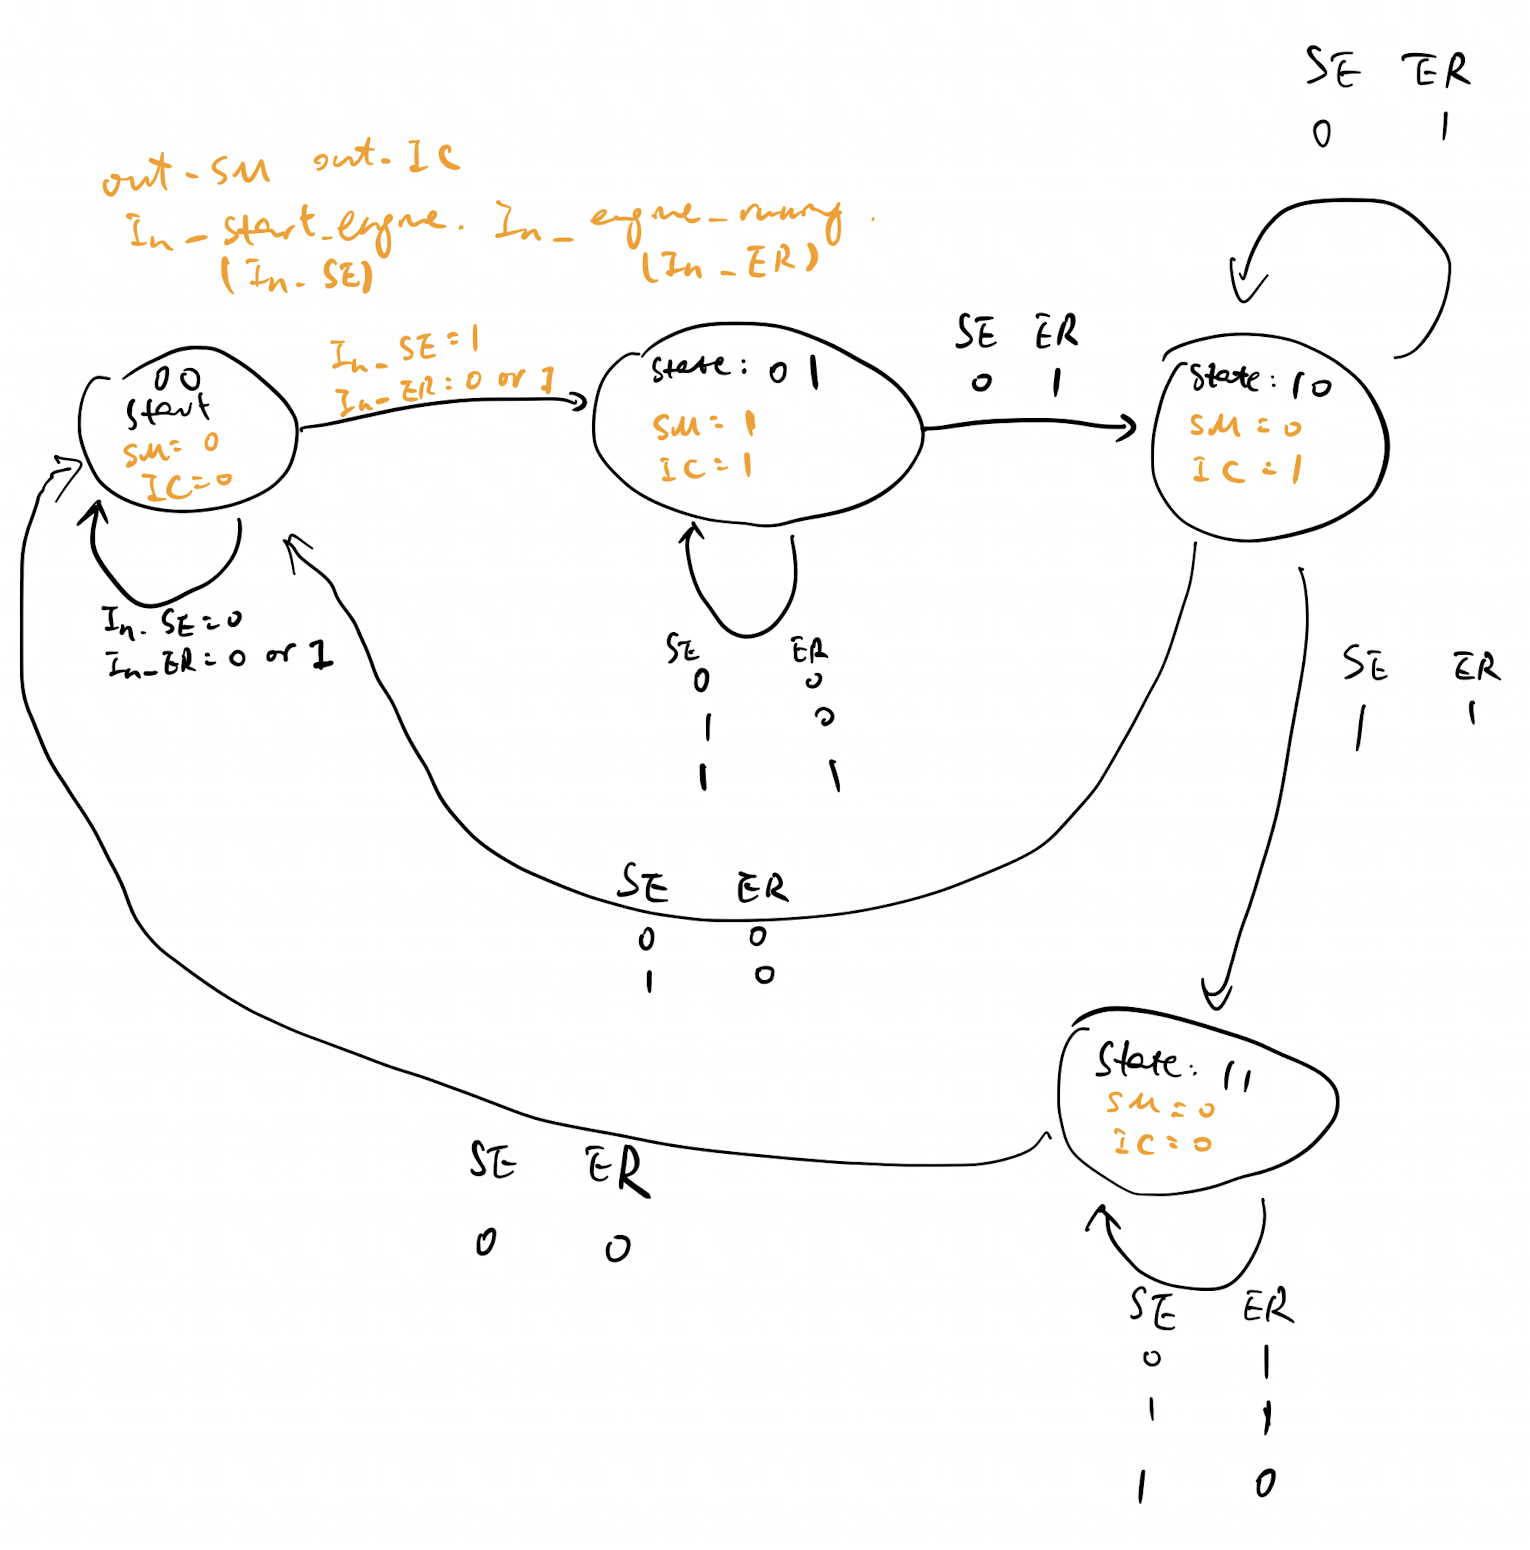
\includegraphics[width=0.8\textwidth]{img/diagram.png}
            \caption{Transition Diagram.}
            \label{fig:diag}
        \end{figure}

        \item[(b)] Draw a truth table for the state transition diagram.

        The truth table is as table~\ref{tab:Q3btruth_table}.
        \begin{table}
            \centering
            \begin{tabular}{cccccccc}
                \toprule
                $q_1$ & $q_0$ & out\_SM & out\_IC & In\_SE & In\_ER & $d_1$ & $d_0$ \\
                \midrule
                0     & 0     & 0       & 0       & 1      & 0      & 0     & 1     \\
                0     & 0     & 0       & 0       & 1      & 1      & 0     & 1     \\
                0     & 0     & 0       & 0       & 0      & 0      & 0     & 0     \\
                0     & 0     & 0       & 0       & 0      & 1      & 0     & 0     \\
                \midrule
                0     & 1     & 1       & 1       & 0      & 0      & 0     & 1     \\
                0     & 1     & 1       & 1       & 1      & 0      & 0     & 1     \\
                0     & 1     & 1       & 1       & 1      & 1      & 0     & 1     \\
                0     & 1     & 1       & 1       & 0      & 1      & 1     & 0     \\
                \midrule
                1     & 0     & 0       & 1       & 0      & 1      & 1     & 0     \\
                1     & 0     & 0       & 1       & 1      & 1      & 1     & 1     \\
                1     & 0     & 0       & 1       & 0      & 0      & 0     & 0     \\
                1     & 0     & 0       & 1       & 1      & 0      & 0     & 0     \\
                \midrule
                1     & 1     & 0       & 0       & 0      & 1      & 1     & 1     \\
                1     & 1     & 0       & 0       & 1      & 1      & 1     & 1     \\
                1     & 1     & 0       & 0       & 1      & 0      & 1     & 1     \\
                1     & 1     & 0       & 0       & 0      & 0      & 0     & 0     \\
                \bottomrule
            \end{tabular}
            \caption{Truth Table for Q3 (b).}
            \label{tab:Q3btruth_table}
        \end{table}

        \item[(c)] Write out the logic expressions for your next-state bits as well as the ouputs \textbf{starter\_motor} and \textbf{ignition\_coil}.
        \begin{equation*}
            \begin{aligned}
                &d_0 = \left( !q_1 \& !q_0 \& \text{In\_SE} \right) | \left( !q_1 \& q_0 \& \left( \text{In\_SE} | !\text{In\_ER} \right) \right) | \left( q_1 \& !q_0 \& \text{In\_SE} \& \text{In\_ER} \right) | \left( q_1 \& q_0 \& \left( \text{In\_SE} | \text{In\_ER} \right) \right) \\
                &d_1 = \left( !q_1 \& q_0 \& !\text{In\_SE} \& \text{In\_ER} \right) | \left( q_1 \& !q_0 \& \text{In\_ER} \right) | \left( q_1 \& q_0 \& \left( \text{In\_SE} | \text{In\_ER} \right) \right)
            \end{aligned}
        \end{equation*}
    \end{enumerate}

\end{document}